
%==============================================================================
% Voorbeeld gebruik documentklasse hogent-article
%==============================================================================
%
% Compileren in TeXstudio:
%
% - Zorg dat Biber de bibliografie compileert (en niet Biblatex)
%   Options > Configure > Build > Default Bibliography Tool: "txs:///biber"
% - F5 om te compileren en het resultaat te bekijken.
% - Als de bibliografie niet zichtbaar is, probeer dan F5 - F8 - F5
%   Met F8 compileer je de bibliografie apart.
%
% Als je JabRef gebruikt voor het bijhouden van de bibliografie, zorg dan
% dat je in ``biblatex''-modus opslaat: File > Switch to BibLaTeX mode.

\documentclass{hogent-article}

%images
\usepackage{graphicx}
\graphicspath{ {./img/} }

%------------------------------------------------------------------------------
% Metadata over het artikel
%------------------------------------------------------------------------------

%---------- Titel & auteur ----------------------------------------------------
\PaperTitle{Heeft de factor muziek invloed op de resultaten van de retrieval practice studiemethode?}
% Dit is typisch de opdracht en het vak waarvoor dit artikel geschreven is, bv.
% ``Verslag onderzoeksproject Onderzoekstechnieken 2018-2019''
\PaperType{Verslag onderzoeksproject Onderzoekstechnieken 2018-2019}

\Authors{Olivier Troch\textsuperscript{1}, Daan Van Vooren \textsuperscript{2}, Robbie Verdurme\textsuperscript{3}, Sebastien Wojtyla\textsuperscript{4}} % Authors



% Als het hier gaat om een voorstel voor de bachelorproef, dan ben je hier
% verplicht de naam van je co-promotor in te vullen. Zoniet, dan kan je het
% leeg laten.
\CoPromotor{}

% Contactinfo: Geef hier de contactgegevens van elke auteur van het artikel (en
% indien van toepassing ook van de co-promotor).
\affiliation{
	\textsuperscript{1} \href{mailto:Olivier.troch.w2257@student.hogent.be}{Olivier.troch.w2257@student.hogent.be}
}
\affiliation{
	\textsuperscript{2} \href{mailto:daan.vanvooren.y1502@student.hogent.be}{daan.vanvooren.y1502@student.hogent.be}
}
\affiliation{
	\textsuperscript{3}
	\href{mailto:robbie.verdurme.y9234@student.hogent.be}{robbie.verdurme.y9234@student.hogent.be}
}
\affiliation{
	\textsuperscript{4}
	\href{mailto;sebastien.wojtyla.y3274@student.hogent.be}{sebastien.wojtyla.y3274@student.hogent.be}
}
%---------- Abstract ----------------------------------------------------------
\Abstract{
	In deze paper werd onderzocht wat de effecten zijn van muziek op de resultaten van de retrieval practice studiemethode.
	In veel studies werd reeds aangetoond dat retrieval practice een goede studiemethode is maar welke factoren hierop een invloed kunnen hebben werd minder besproken. De paper gaat dieper in op deze vraag door te onderzoeken of het beluisteren van muziek gedurende de retrieval practice methode enige invloed heeft op de resultaten.
	Het te verwachten resultaat is dat het beluisteren van muziek tijdens de retrieval practice studiemethode een negatief effect zal hebben. Deze paper kan bijdragen aan verder onderzoek van de retrieval practice methode.
}

%---------- Onderzoeksdomein en sleutelwoorden --------------------------------
\Keywords{Onderzoeksproces, Studiemethodes, Retrieval Practice}
\newcommand{\keywordname}{Sleutelwoorden} % Defines the keywords heading name

%---------- Titel, inhoud -----------------------------------------------------

\begin{document}
	
	\flushbottom % Makes all text pages the same height
	\maketitle % Print the title and abstract box
	\tableofcontents % Print the contents section
	\thispagestyle{empty} % Removes page numbering from the first page
	
	%------------------------------------------------------------------------------
	% Hoofdtekst
	%------------------------------------------------------------------------------
	
	\section{Inleiding} %inleiding over retrieval practice + paper
	Retrieval practice is een studiemethode die ervoor zorgt dat leerstof langer onthouden kan worden op lange termijn. Hoewel reeds aangetoond werd dat dit een effectieve methode is voor het studeren verwachtten wij een ander resultaat wanneer we een variabele aanpassen. De variabele die wij hebben onderzocht in deze paper is het effect van muziek in combinatie met retrieval practice tijdens het instuderen van een tekst.
	
	\section{Overzicht literatuur} % literatuurstudie
	
	% Refereren naar de literatuur kan met:
	% \autocite{BIBTEXKEY} -> (Auteur, jaartal)
	% \textcite{BIBTEXKEY} -> Auteur (jaartal)
	% Voorbeeld van een referentie~\autocite{Moore2002}
	
	
	
	\section{Methodologie} %0 hypothese
	De variabele die getest werd in deze paper is het effect van het beluisteren van muziek tijdens de retrieval practice methode.
	Door het beluisteren van muziek tijdens het instuderen kan het brein meer gestimuleerd worden ofwel worden afgeleid. Afhankelijk van de persoon zal de muziek een positief of negatief effect hebben. Bij sommigen zal dit helpen om de studiematerie te kunnen linken aan de muziek en deze zo gemakkelijker te onthouden terwijl bij andere personen deze kan afleiden waardoor ze zich concentreren op de muziek en niet de te onthouden materie.Dit kan een grote invloed hebben op het studeren zoals reeds bewezen is \autocite{ChanEtAl1998}.
	


	
	\section{Experimenten} %hoe we de experimenten uitvoeren
	Tijdens het onderzoek kreeg iedere informaticastudent een tekst over Darwin die hij/zij moest bestuderen. Vervolgens werden de studenten opgesplitst in vier subgroepen. Elke subgroep werd gedifferentieerd op basis van het wel of niet luisteren naar muziek en het wel of niet toepassen van de retrieval practice methode.
	De eerste subgroep heeft de standaard retrieval practice methode toegepast zonder aangepaste variabele. 

	De tweede subgroep heeft naar muziek geluisterd tijdens het instuderen van de tekst. In combinatie met deze variable werd er nog steeds gewerkt met de retrieval practice methode.
	
	De derde subgroep heeft ook naar muziek geluisterd tijdens het instuderen van de tekst maar zonder het toepassen van de retrieval practice methode.
	
	De vierde kreeg geen muziek te horen krijgen tijdens het instuderen van de tekst en ging dan ook niet te werk aan de hand van de retrieval practice methode.
	
	Hierdoor kan nagegaan worden of de variabele een invloed heeft op het studeren van een tekst aan de hand van de retrieval practice methode. Merk op dat we elke tweedejaars informaticastudent er toe verplichtten om deel te nemen aan deze test waardoor het resultaat niet op de hele groep studenten toepasbaar is zonder enig foutpercentage \autocite{karpicke2009metacognitive}.
	
	\section{Verwachtingen} %wat we verwachten van de experimenten
	We veronderstelden dat de eerste subgroep analoge resultaten ging behalen aan de resultaten uit de artikels over de retrieval practice methode \autocite{butler2010repeated, pyc2012test, karpicke2007repeated, karpicke2008critical}. Dit omdat deze methode reeds vaak getest werd in verschillende experimenten. Zoals volgende boxplotten aantonen
%rt
	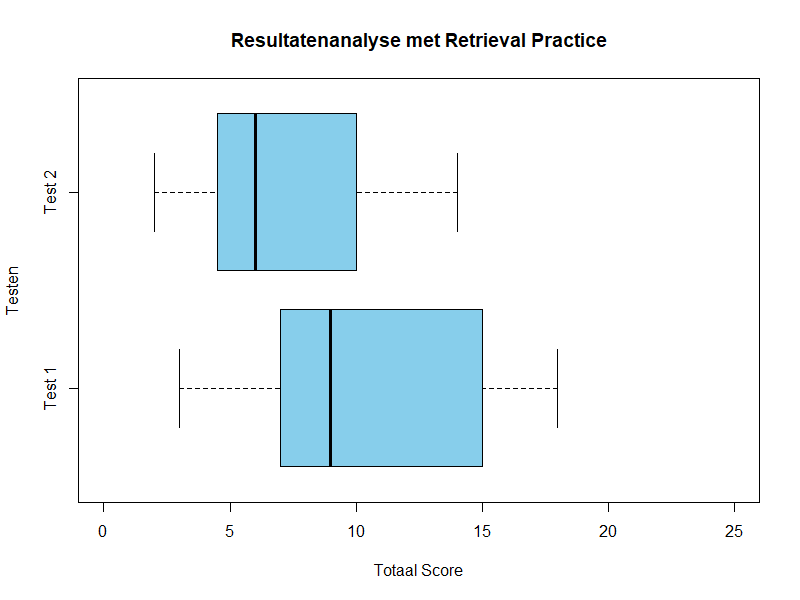
\includegraphics[width=120px]{Verwacht_RetrievalPractice}
	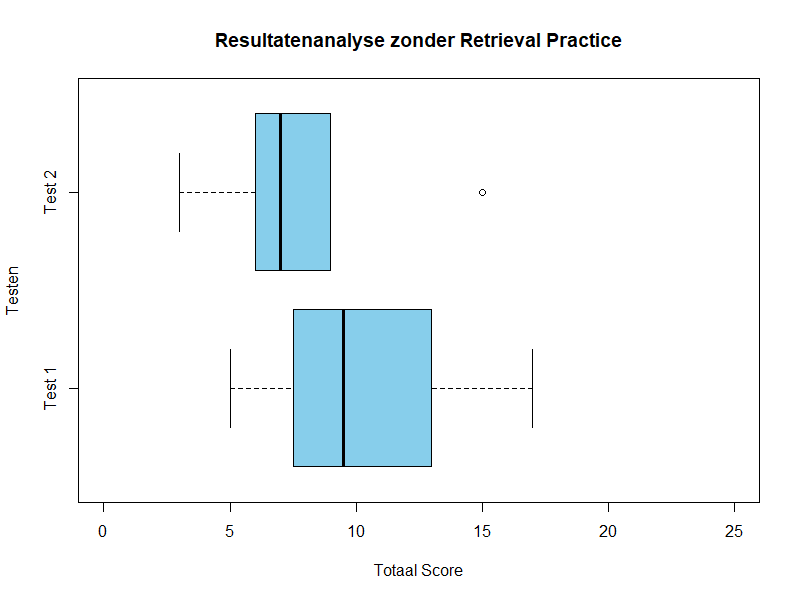
\includegraphics[width=120px]{Verwacht_ZonderRetrievalPractice}
%rt per score
	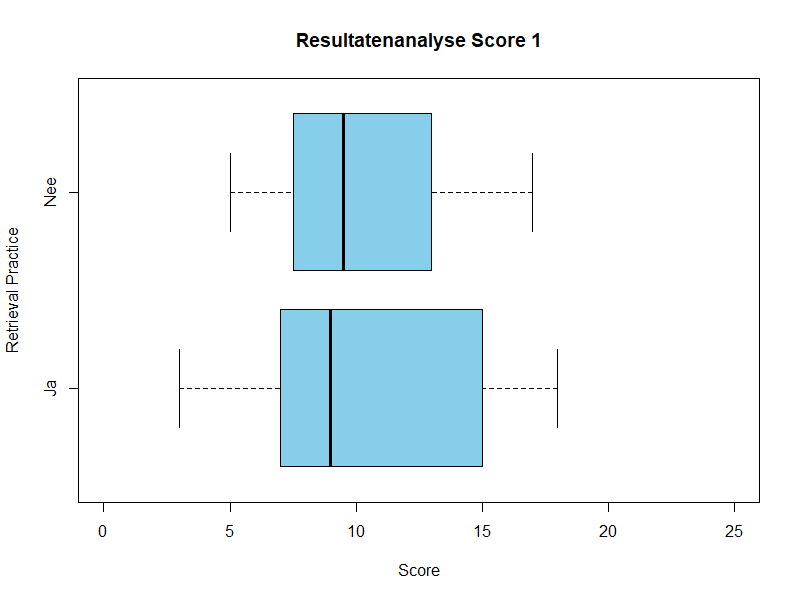
\includegraphics[width=120px]{Verwacht_RT_Score1}
	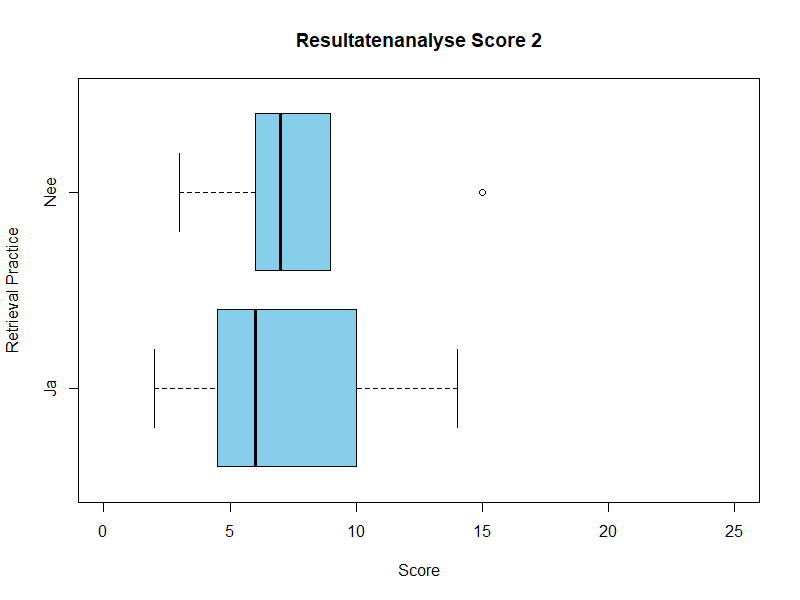
\includegraphics[width=120px]{Verwacht_RT_Score2}
	
%table gemiddelde
	\begin{tabular}{ |p{10em}|c|c| }
	\hline
		\multicolumn{3}{|c|}{Gemiddelde} \\
	\hline
		& Test 1 & Test 2 \\
	\hline
		Met Retrieval Practice & 10.375 & 7.125 \\
		Zonder Retrieval Practice & 10.25 & 7.75 \\
	\hline
	\end{tabular}
	
	%table standaardafwijking
	\begin{tabular}{ |p{10em}|c|c| }
	\hline
		\multicolumn{3}{|c|}{Standaardafwijking} \\
	\hline
		& Test 1 & Test 2 \\
	\hline
		Met Retrieval Practice & 5.153016 & 4.257347 \\
		Zonder Retrieval Practice & 3.918819 & 3.494894 \\
	\hline
	\end{tabular}
	
	Daarnaast verwachtten we dat het beluisteren van muziek een negatief effect ging hebben op het resultaat. Door het beluisteren van muziek kan je sneller afgeleid geraken tijdens het lezen van de tekst en deze dan ook minder gemakkelijk onthouden. Zoals de boxplotten hieronder illustreren hebben de groepen die naar muziek luisterden tijdens het studeren minder gescoort dan de groepen die niet naar muziek luisterden.
%muziek
	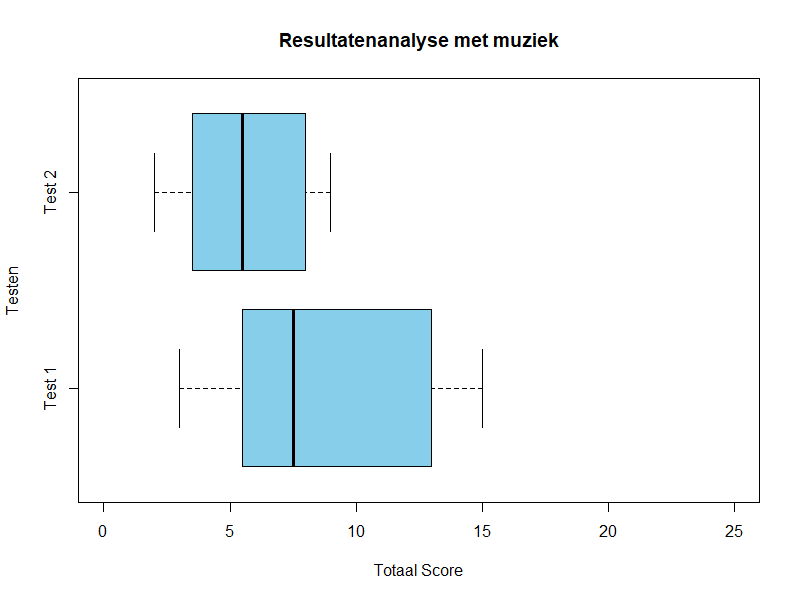
\includegraphics[width=120px]{Verwacht_Muziek}
	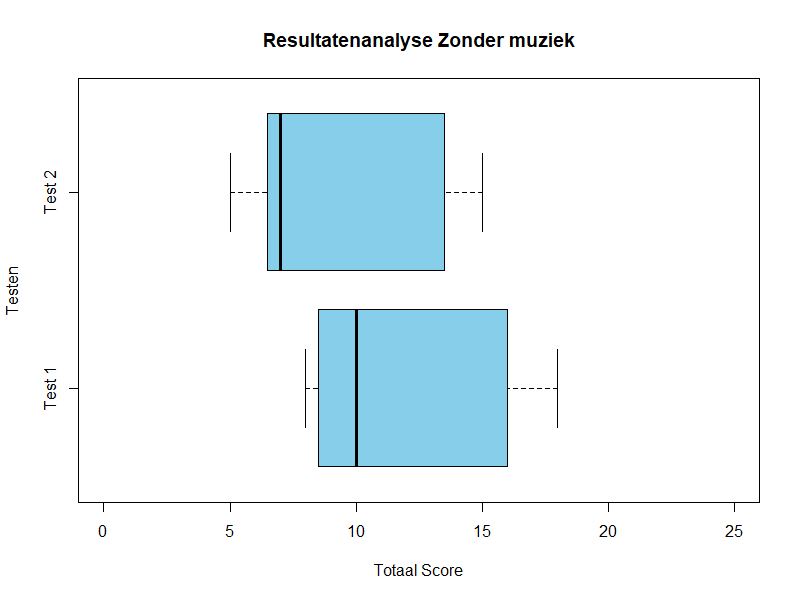
\includegraphics[width=120px]{Verwacht_ZonderMuziek}
	
%muziek per score
	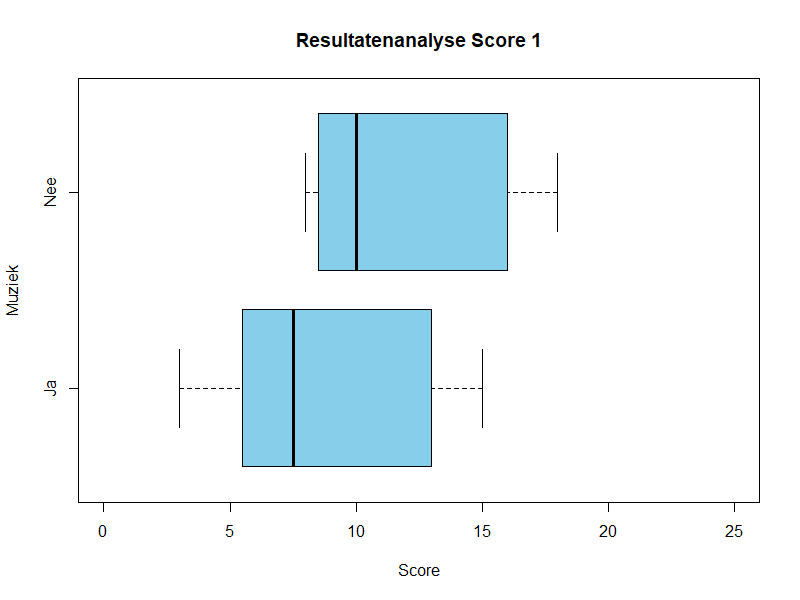
\includegraphics[width=120px]{Verwacht_Muziek_Score1}
	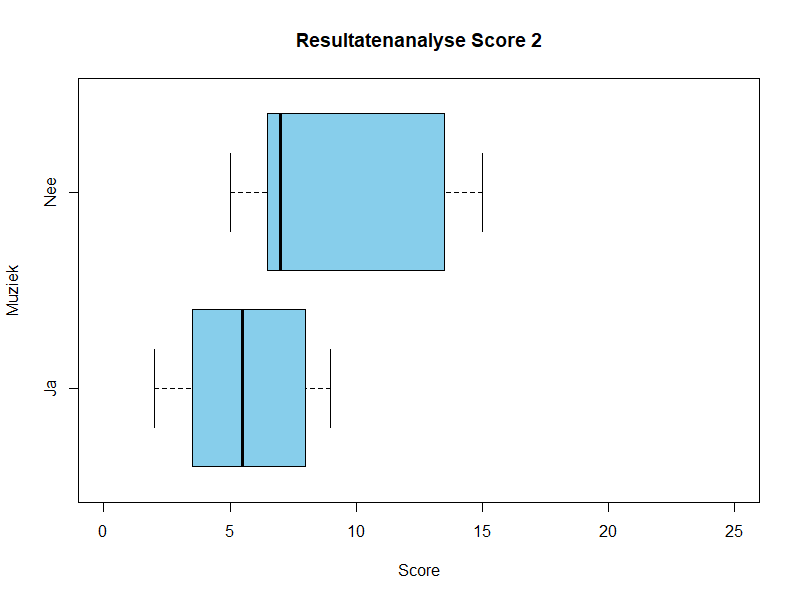
\includegraphics[width=120px]{Verwacht_Muziek_Score2}
	
	%table gemiddelde
	\begin{tabular}{ |p{10em}|c|c| }
	\hline
		\multicolumn{3}{|c|}{Gemiddelde} \\
	\hline
		& Test 1 & Test 2 \\
	\hline
		Met Muziek & 8.75  & 5.625 \\
		Zonder Muziek & 11.875 & 9.25 \\
	\hline
	\end{tabular}
	
	%table standaardafwijking
	\begin{tabular}{ |p{10em}|c|c| }
	\hline
		\multicolumn{3}{|c|}{Standaardafwijking} \\
	\hline
		& Test 1 & Test 2 \\
	\hline
		Met Muziek & 4.399675  & 2.615203 \\
		Zonder Muziek & 4.120940 & 4.026697 \\
	\hline
	\end{tabular}
	
	Als we de verwachtingen op alle variablen toepassen zien we heel duidelijk dat de methode met retrieval practice en zonder muziek de beste is. Dit komt omdat het beluisteren van muziek afleidend is waardoor de efficiëntie van de retrieval practice studie methode daalt. 
	%rt en muziek
	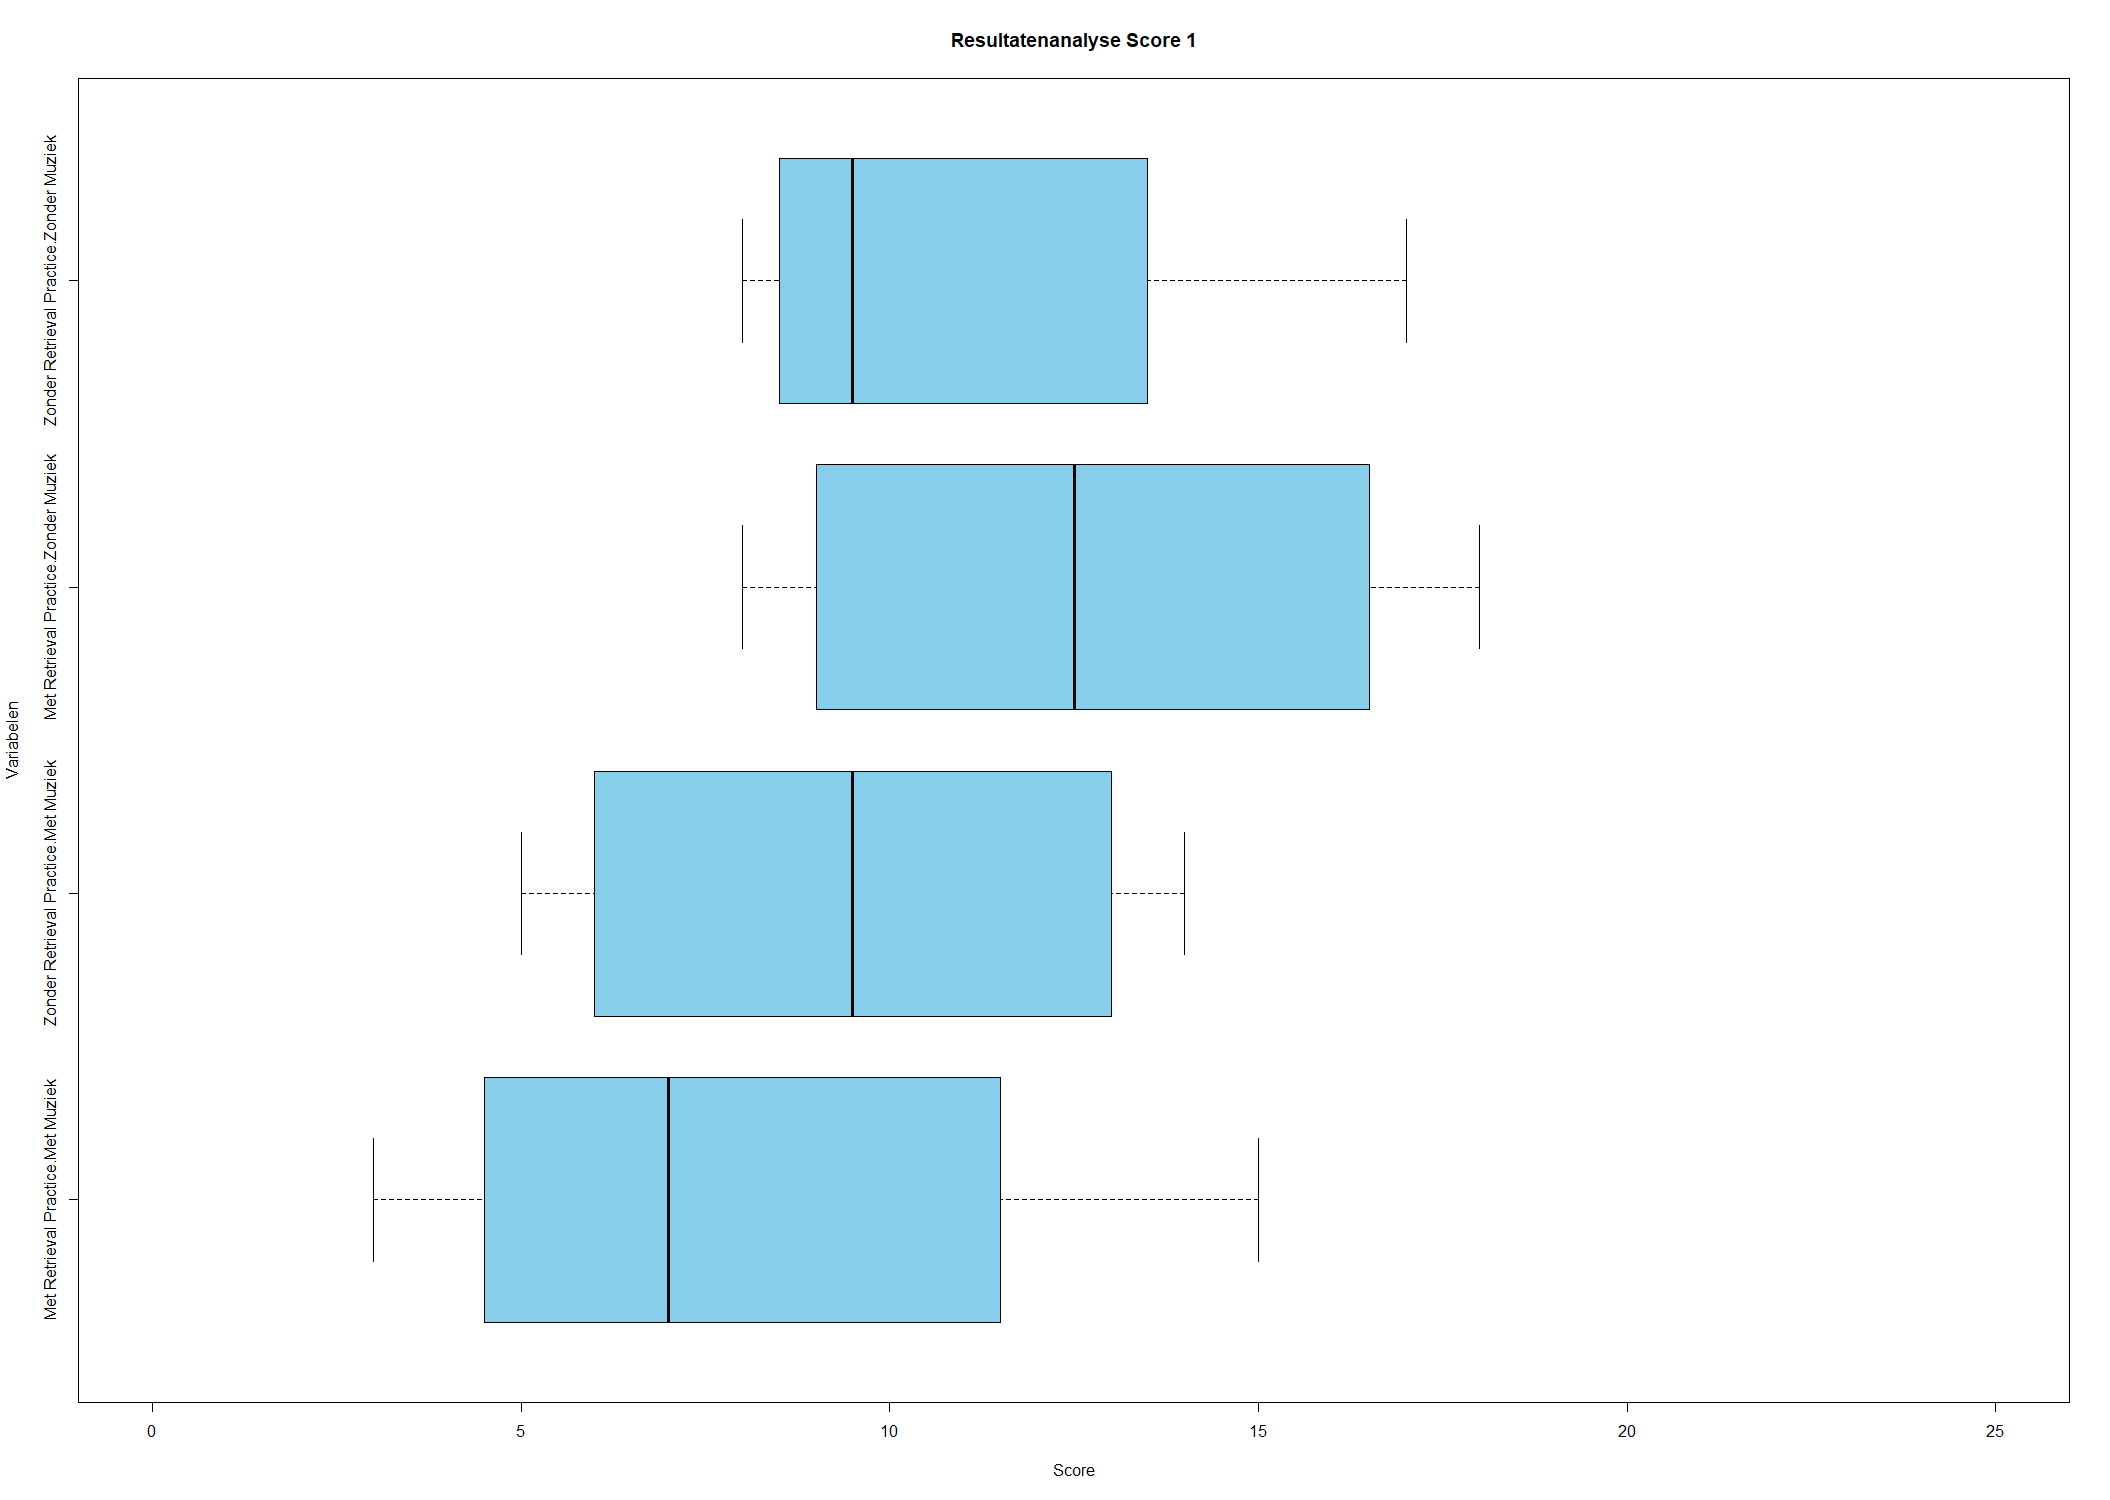
\includegraphics[width=250px]{Verwacht_MuziekRT_Score1}
	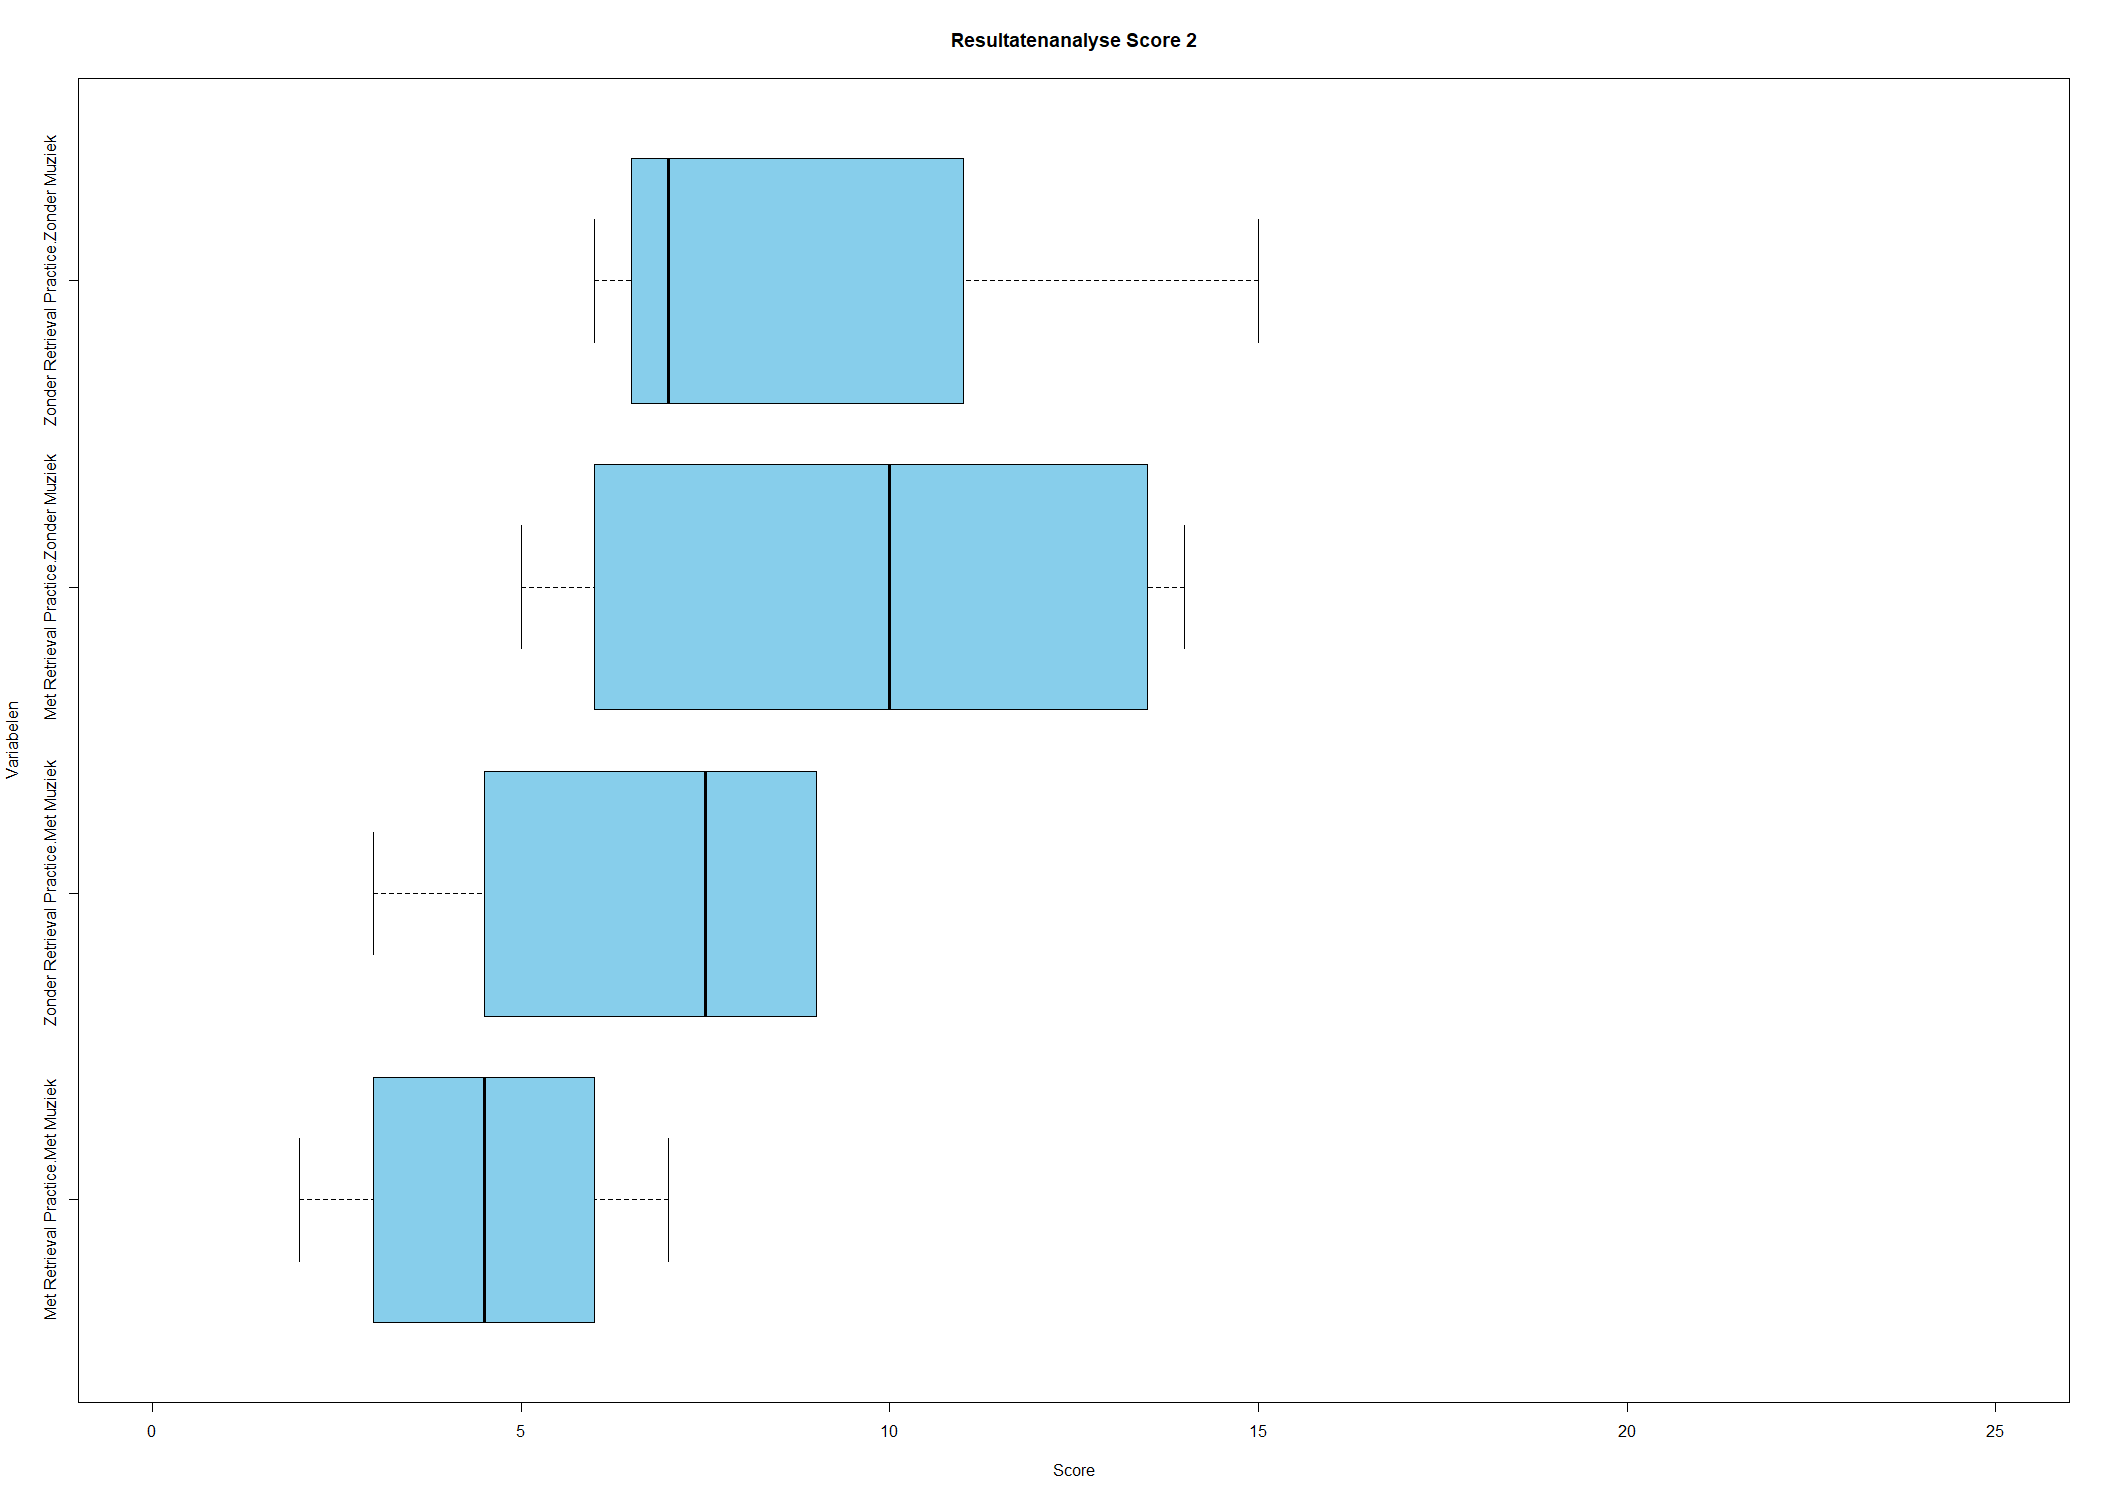
\includegraphics[width=250px]{Verwacht_MuziekRT_Score2}
	%table gemiddelde
	\begin{tabular}{ |p{10em}|c|c| }
	\hline
		\multicolumn{3}{|c|}{Gemiddelde} \\
	\hline
		& Test 1 & Test 2 \\
	\hline
		Met Retrieval Practice Met Muziek  & 8 & 4.5 \\
	\hline
		Zonder Retrieval Practice Met Muziek & 6.75 & 6.75 \\
	\hline
		Met Retrieval Practice Zonder Muziek & 12.75  & 9.75 \\
	\hline
		Zonder Retrieval Practice Zonder Muziek & 11 & 8.75 \\
	\hline
	\end{tabular}
	
	%table standaardafwijking
	\begin{tabular}{ |p{10em}|c|c| }
	\hline
		\multicolumn{3}{|c|}{Standaardafwijking} \\
	\hline
		& Test 1 & Test 2 \\
	\hline
		Met Retrieval Practice Met Muziek  & 5.09902 & 2.081666 \\
	\hline
		Zonder Retrieval Practice Met Muziek & 2.872281 & 2.872281 \\
	\hline
		Met Retrieval Practice Zonder Muziek & 4.573474  & 4.425306 \\
	\hline
		Zonder Retrieval Practice Zonder Muziek & 4.082483 & 4.193249 \\
	\hline
	\end{tabular}
			
	\section{Analyse resultaten} %bespreken van resultaten
	\subsection{Retrieval Practice} 
	In vergelijking met de artikels over de retrieval practice \autocite{butler2010repeated, pyc2012test, karpicke2007repeated, karpicke2008critical} liggen onze uitslagen dicht bij die van de artikels over de retrieval practice. Dit houdt in dat we kunnen bewijzen dat de retrieval practice een aangeraden studiemethode is met een hoge studie efficiëntie.
	
	%met rt en zonder rt vergelijken
	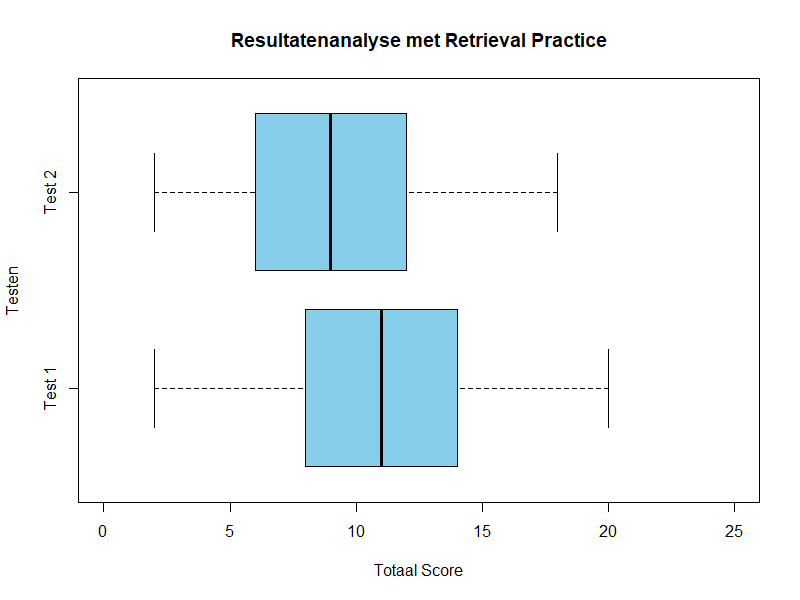
\includegraphics[width=120px]{Rplot_MetRetrievalPractice}
	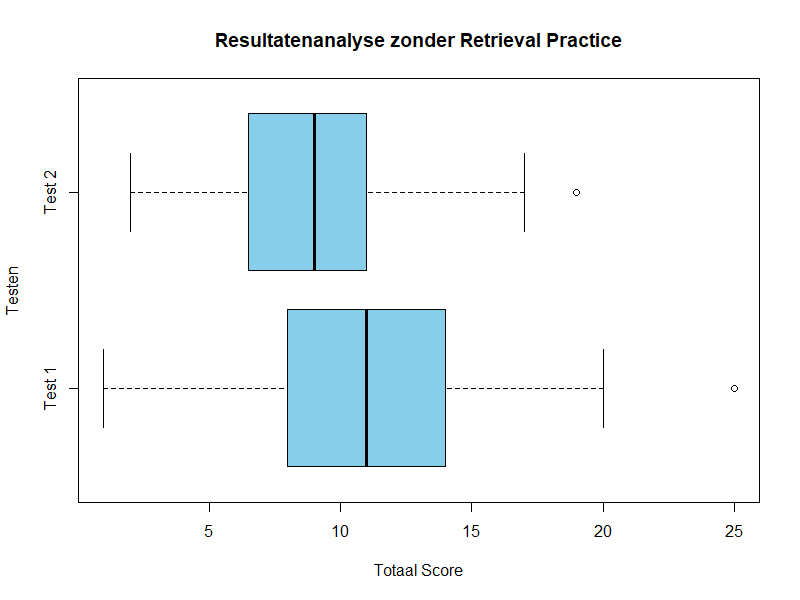
\includegraphics[width=120px]{Rplot_ZonderRetrievalPractice}
	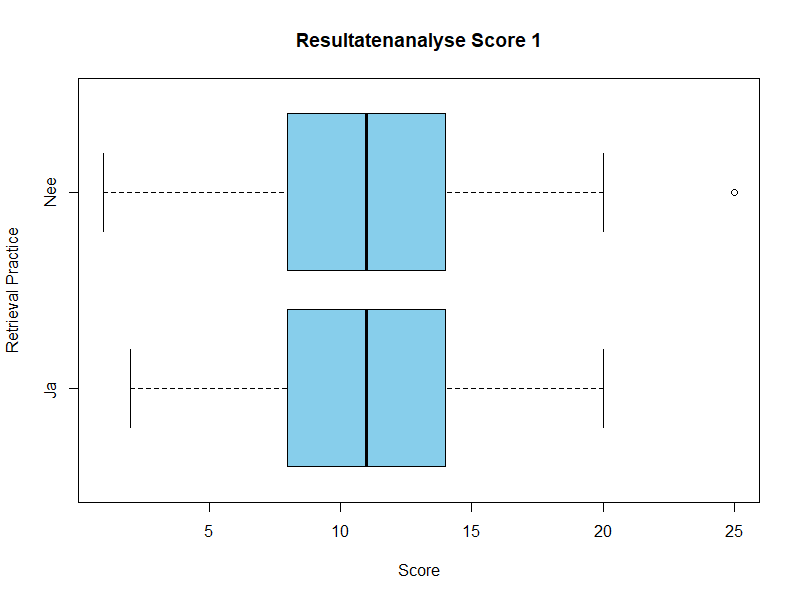
\includegraphics[width=120px]{Rplot_RetrievalPractice_Score1}
	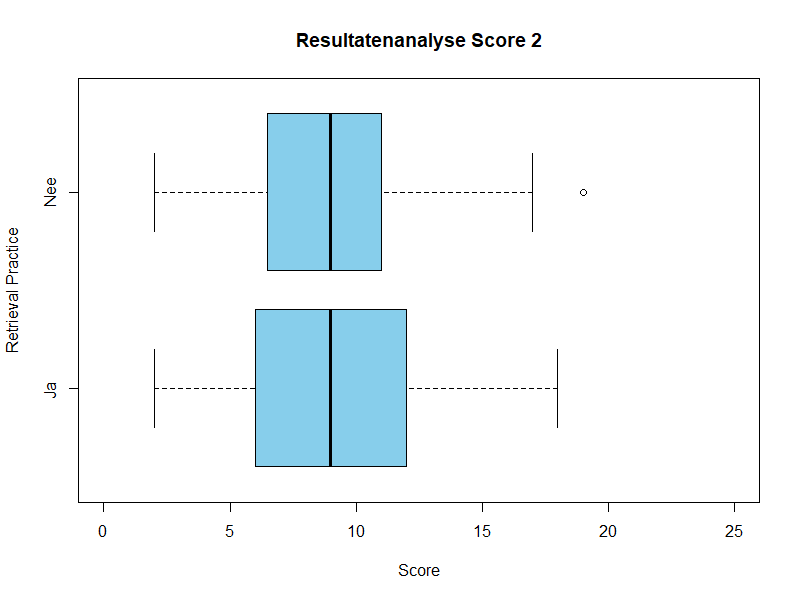
\includegraphics[width=120px]{Rplot_RetrievalPractice_Score2}
	
	%table gemiddelde
	\begin{tabular}{ |p{10em}|c|c| }
		\hline
			\multicolumn{3}{|c|}{Gemiddelde} \\
		\hline
			& Test 1 & Test 2 \\
		\hline
			Met Retrieval Practice & 11.0303 & 9.077778 \\
			Zonder Retrieval Practice & 11.45455 & 9.15 \\
		\hline
	\end{tabular}

	%table standaardafwijking
	\begin{tabular}{ |p{10em}|c|c| }
	\hline
		\multicolumn{3}{|c|}{Standaardafwijking} \\
	\hline
		& Test 1 & Test 2 \\
	\hline
		Met Retrieval Practice & 4.348245 & 4.025837 \\
		Zonder Retrieval Practice & 4.471902 & 3.913948 \\
	\hline
	\end{tabular}
	
	%tekst Retrieval practice
	Vanuit de testen blijkt dat tussen de groep die de retrieval practice methode toepaste en de groep die dit niet deed de score niet significant verschillend is. De groep die de retrieval practice toepaste had net iets minder onthouden van de ingestudeerde tekst. Dit valt binnen het foutpercentage. Hierdoor kunnen we enzigsins bevestigen dat de retrieval practice studie methode een efficiënte studie methode is zoals al werd beweerd in de opgezochte artikels. Hiernaast hebben we bij onze test geen significant verschil gevonden tussen het gebruik van deze studie methode en een eigen studie methode.
	
	\subsection{Muziek}
	%met muziek en zonder muziek vergelijken
	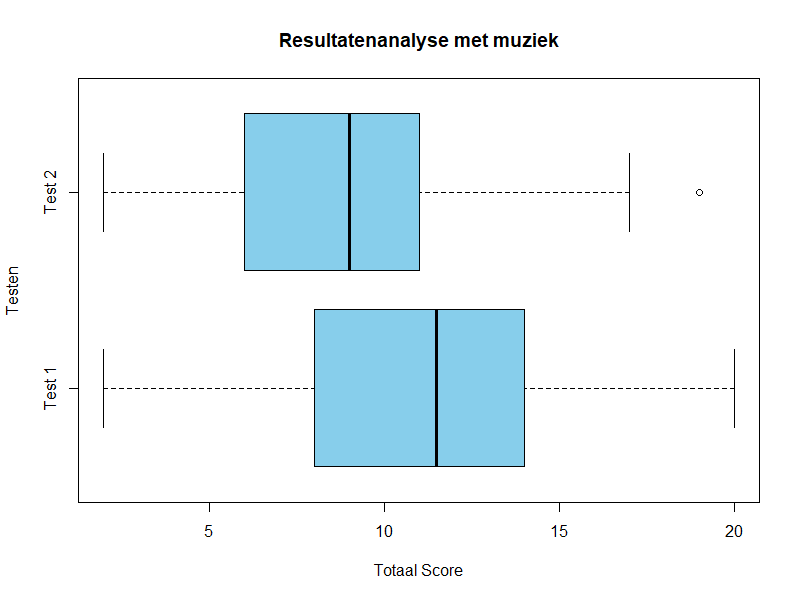
\includegraphics[width=120px]{Rplot_MetMuziek}	
	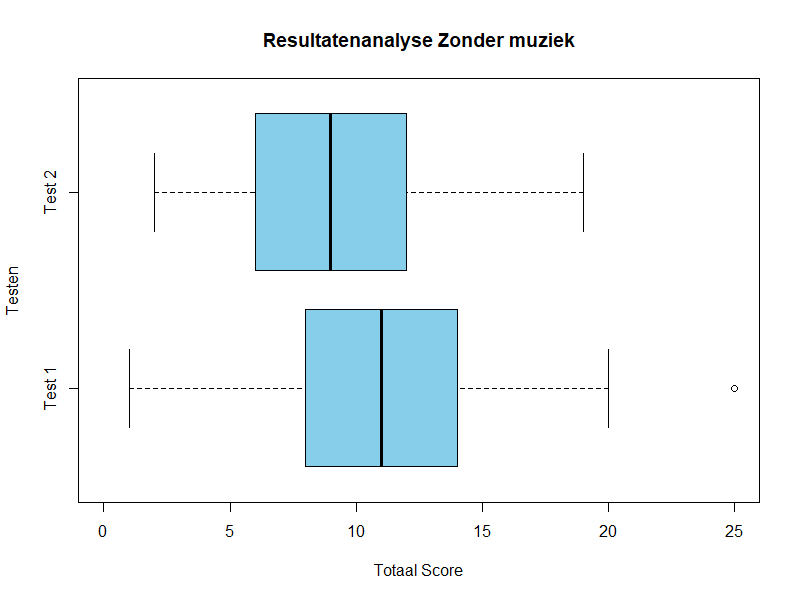
\includegraphics[width=120px]{Rplot_ZonderMuziek}
	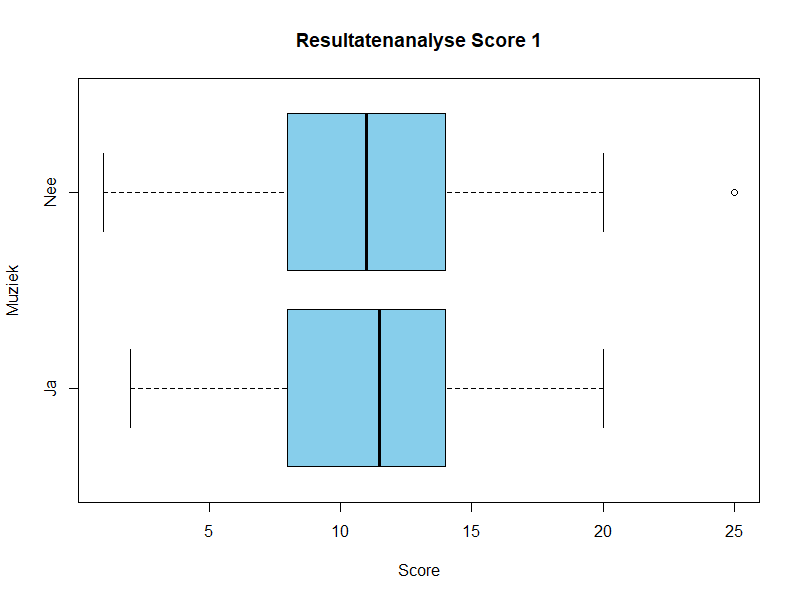
\includegraphics[width=120px]{Rplot_Muziek_Score1}
	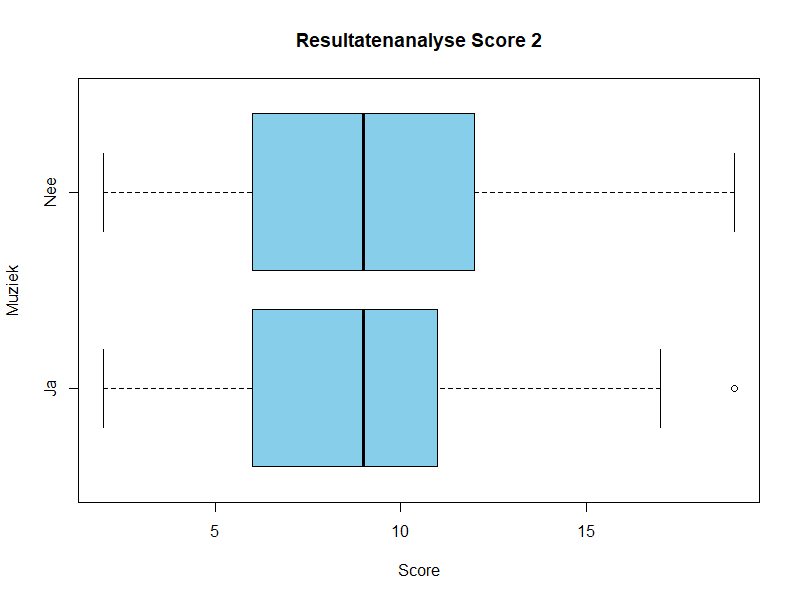
\includegraphics[width=120px]{Rplot_Muziek_Score2}
	
	%table gemiddelde
	\begin{tabular}{ |p{10em}|c|c| }
	\hline
		\multicolumn{3}{|c|}{Gemiddelde} \\
	\hline
		& Test 1 & Test 2 \\
	\hline
		Met Muziek & 11.36047 & 8.988764 \\
		Zonder Muziek & 11.11881 & 9.246914 \\
	\hline
	\end{tabular}

	%table standaarafwijking
	\begin{tabular}{ |p{10em}|c|c| }
	\hline
		\multicolumn{3}{|c|}{Standaardafwijking} \\
	\hline
		& Test 1 & Test 2 \\
	\hline
		Met Muziek & 4.429614 & 3.797411 \\
		Zonder Muziek & 4.393830 & 4.154909 \\
	\hline
	\end{tabular}

	%tekst muziek
	Verder hebben we in deze paper gekeken naar de impact van het beluisteren van muziek tijdens het studeren. Uit de testen die we afgenomen hebben, blijkt er geen significant verschil te zijn. Dit was niet zoals we verwacht hadden alvoor we aan de testen begonnen. Dit valt eventueel te veklaren omdat de testpersonen het beluisteren van muziek al reeds opgenomen hebben in hun eigen studemethodes
	
	\subsection{Retieval Practice met Muziek}
	%met rt en muziek vergelijken
	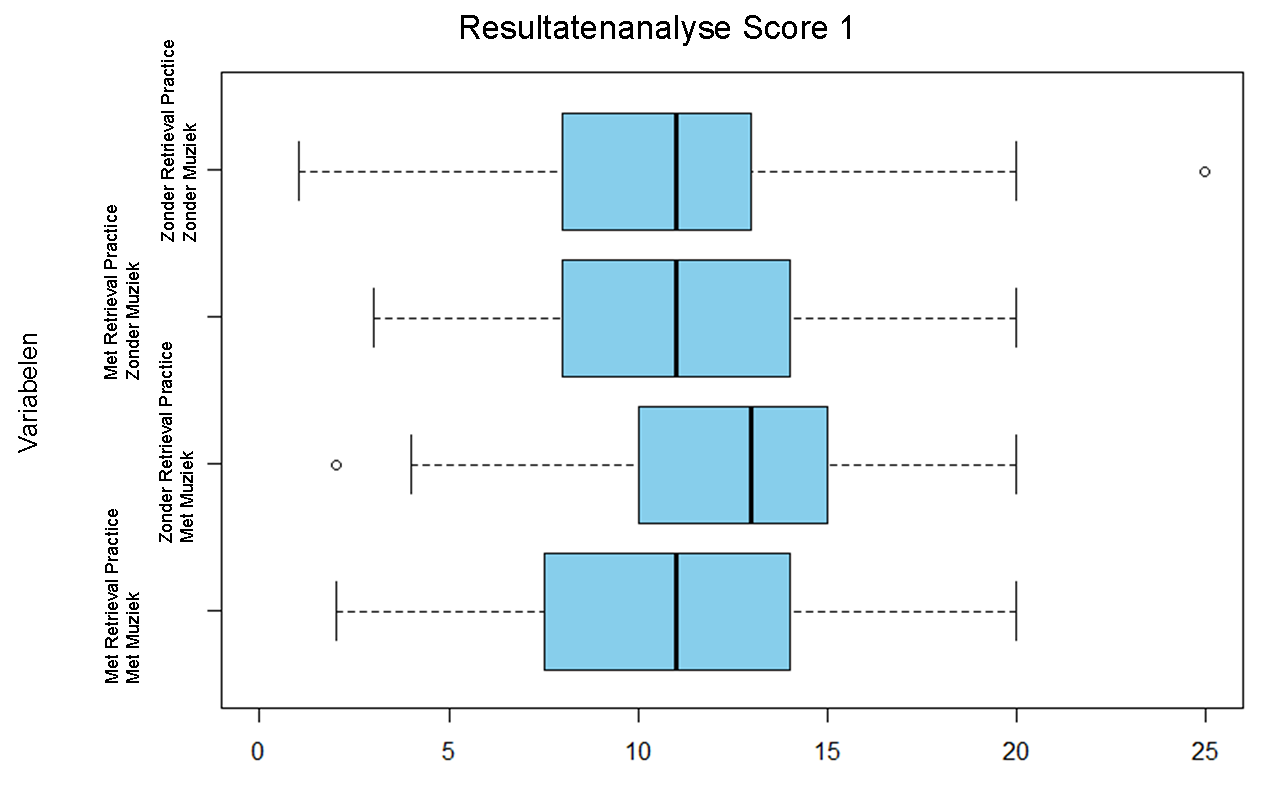
\includegraphics[width=250px]{Final_boxplots_Score1}
	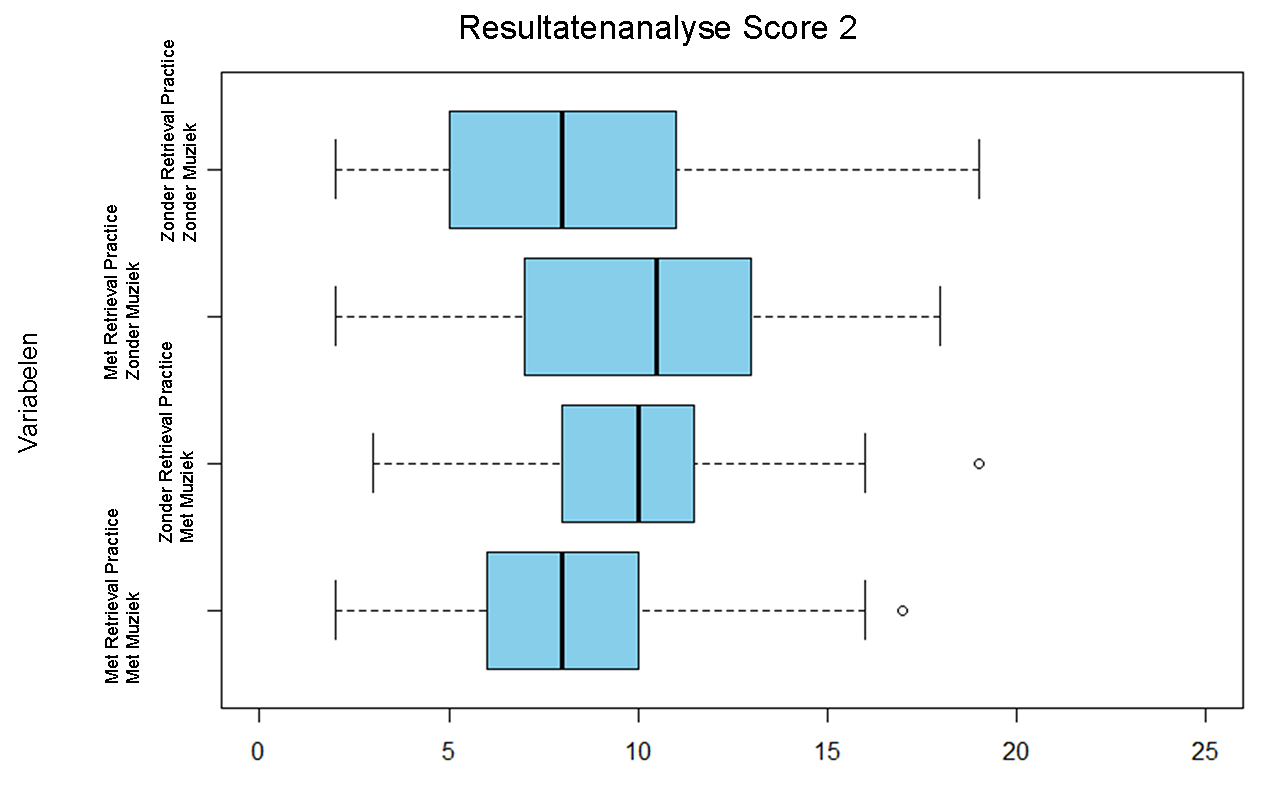
\includegraphics[width=250px]{Final_boxplots_Score2}
	
	%table gemiddelde
	\begin{tabular}{ |p{10em}|c|c| }
	\hline
		\multicolumn{3}{|c|}{Gemiddelde} \\
	\hline
		& Test 1 & Test 2 \\
	\hline
		Met Retrieval Practice Met Muziek  & 10.55556 & 8.714286 \\
	\hline
		Zonder Retrieval Practice Met Muziek & 11.6087 & 9.190476 \\
	\hline
		Met Retrieval Practice Zonder Muziek & 11.6 & 9.512195 \\
	\hline
		Zonder Retrieval Practice Zonder Muziek & 11.28571 & 9.105263 \\
	\hline
	\end{tabular}

	%table standaardafwijking
	\begin{tabular}{ |p{10em} |c|c| }
	\hline
		\multicolumn{3}{|c|}{Standaardafwijking} \\
	\hline
		& Test 1 & Test 2 \\
	\hline
		Met Retrieval Practice Met Muziek  & 4.411249 & 3.8676\\
	\hline
		Zonder Retrieval Practice Met Muziek & 4.31266 & 4.284049 \\
	\hline
		Met Retrieval Practice Zonder Muziek & 4.250134  & 4.213798\\
	\hline
		Zonder Retrieval Practice Zonder Muziek & 4.6867 & 3.516674 \\
	\hline
	\end{tabular}
	
	Deze boxplotten zijn enigzins wat we verwacht hadden in deze paper. Namelijk dat het instuderen met de retrieval practice zonder muziek een positief resultaat heeft. Terwijl studeren met muziek en zonder retrieval practice dan weer een eerder positief resultaat heeft tegenover studeren met muziek en met retrieval practice. Dit kunnen we eventueel verklaren door dat de testpersoon de tekst kan koppelen aan de muziek omdat hij zich enkel focust op het lezen en de muziek en niet op het noteren. Wanneer retrieval practice en muziek toch samengevoegd worden, kan dit eventueel voor verwarring zorgen. Dit blijkt ook zo te zijn als je de resultaten bekijkt. 
	
	\section{Conclusie}
	Uit de resultaten van deze paper kunnen we concluderen dat de retrieval practice een efficiënte studiemethode is. Dit is meermaals bewezen in verschillende papers. Net zoals in die papers hebben wij hetzelfde resultaat, namelijk dat de groep die de retrieval practice zonder het luisteren van muziek het beste scoort op onze test.
	
	Verder kunnen we nog een paar conclusies afleiden van de resultaten, namelijk dat de eigen studie methode(zonder retrieval practice) en met muziek als tweede beste uit onze test komt. Dit kan op verschillende manieren verklaard worden. Een van deze manieren is dat de studenten in kwestie dit eventueel al gewoon zijn en het beluisteren van muziek al reeds opgenomen is in hun studiemethode. 
	
	Zoals als reeds besproken in deze conclusie kunnen we onze methodologie verwerpen. Dit is omdat er geen significant verschil gevonden is tussen het beluisteren van muziek tijdens het instuderen en het bestuderen van de tekst zonder het beluisteren van muziek.
	
	
	\section{Opmerkingen}
	De verbeterings criteria werden niet op voorhand meegegeven aan de studenten. Dit heeft enigzins wel invloed op de resultaten. Hierdoor weten de studenten niet precies op wat ze moeten letten bij het instuderen van de tekst.
	Verder hebben we de informaticastudenten verplicht om de retrieval practice methode toe te passen in plaats van hun eigen studiemethodes die de testpersonen al reeds kennen en gebruiken in het dagelijkse leven. Dit kan ook een negatief effect hebben.
	Een volgende opmerking is dat alle variablen in deze test invloed hebben op het resultaat. Dit gaat over de variablen die de andere groepen van informatica opgenomen hebben. Deze zijn niet opgenomen in deze paper maar wel tijdens de test. Deze heeft enigzins invloed op het resultaat.
	Als laaste opmerking wil ik nog vermelden dat de test chaotisch verlopen is en de informaticastudenten niet altijd wisten wat nu juist de bedoeling was. Om die reden kunnen er fouten in de testen zitten. 
	Hierdoor kunnen we niets concluderen uit de resultaten van deze paper.
	
	%------------------------------------------------------------------------------
	% Referentielijst
	%------------------------------------------------------------------------------
	% voorkomen. Gebruik JabRef om je bibliografie bij te houden en vergeet niet
	% om compatibiliteit met Biber/BibLaTeX aan te zetten (File > Switch to
	% BibLaTeX mode)
	
	\phantomsection
	\printbibliography[heading=bibintoc]
	
\end{document}
